% !TEX encoding = UTF-8 Unicode
% !TEX root = rapport.tex

\part{Initiatives et solutions}\label{initiatives_actuelles}

\chapter{Initiatives des pouvoirs publics}
\label{chap:initialivespublic}

\section{Mesures des pouvoirs publics français}

Les pouvoirs publics ne sont bien sûr pas totalement sourds aux
problèmes que rencontre aujourd'hui le système éducatif. Nous allons
nous intéresser tout d'abord au \og{}B2i et C2i\fg{} qui tentent de répondre aux
problèmes de contenu puis aux opérations \og{}ordinateurs
portables\fg{} qui visent une intégration des \gls{ntic} dans les méthodes
d'apprentissages. Nous finirons par l'analyse rapide d'un
rapport : \og{}Refondons l'école de la république\fg{}
demandé par le gouvernement Ayrault.
% todo : deuxième rapport ?

\subsection{Le B2i et C2i}
Mis en place à partir de la rentrée universitaire 2003
\cite{circulaire_c2i}, le brevet informatique et internet (B2i) et le
certificat informatique et internet (C2i) 
visent à encadrer la formation des élèves et étudiants aux technologies
informatisées et à internet par l'établissement d'un socle commun.

\begin{figure}[H]
	\begin{center}
	\makebox[\textwidth]{
		\includegraphics[width=1.4\textwidth]{../resources/illustrations/c2i}
	}
	\caption{Différents niveaux et spécialités du B2i et C2i}
	\end{center}
\end{figure}


Cette initiative vise à mettre en place une formation nationale des
étudiants aux \gls{ntic}\cite{b2i_c2i}. Cette formation se fait de l'école élémentaire
jusqu'au lycée par le B2i puis se poursuit dans les universités avec
le C2i. Ces différents niveaux de brevets et certificats se
matérialisent pour chaque niveau par une liste de compétences que
l'élève ou l'étudiant doit posséder. Il appartient ensuite aux écoles
et aux universités d'organiser la formation, le contrôle des
connaissances et la remise de ces brevets et certificats. Il serait
fort intéressant et sûrement très instructif d'étudier comment ce
dispositif est intégré chez les différents acteurs (école, collège,
lycée, université). Étudier quels sont les modes d'enseignement et
les modalités d'évaluation\ldots

\subsection{Les opérations "ordinateurs portables"}

Les opérations \og{}ordinateurs portables\fg{} sont à la mode au
lycée. OrdiLib' en Midi-Pyrénées, Ordipass en Pays de la Loire, LoRdi
en Languedoc-Roussilon, ces initiatives des régions visent à fournir à
chaque collégien ou lycéen l'accès à un ordinateur portable personnel.

Afin d'étudier l'impact que peut avoir ce type d'action nous allons
nous pencher, entre autres, sur le cas de l'opération \og{}Un collégien, un
ordinateur portable\fg{} qui fût mise en place par le conseil régional
des Landes en septembre 2001\cite{portables40}. 

\begin{figure}[h]
	\begin{center}
		\includegraphics[width=\textwidth]{../resources/illustrations/usage_portables_without_caption}
	\caption{Étude d'évaluation de l'opération \og Un collégien,
          un ordinateur portable \fg{} pour le Conseil général des
          Landes, 2008--2009. Taux d'utilisation.}
		\label{fig:graph_op_portables}
        \end{center}
\end{figure}

Il semble selon le graphique \ref{fig:graph_op_portables}\cite{portables60}, que
60\% des élèves et 57\% des professeurs se servent au moins un jour
sur deux ce qui semble plutôt encourageant. Cependant, il est
intéressant de s'interroger sur l'utilisation qui en est faite. Selon
le graphique \ref{fig:graph_op_portables2}, il en ressort que
l'ordinateur est principalement utilisé par les élèves pour
récupérer ou présenter des documents et faire des exercices. Il semble
donc que les méthodes pédagogique ne soit pas bouleversé par l'arrivée
de l'informatique mais au contraire que la pédagogie traditionnel
s'adapte aux nouveaux supports. Nous pensons qu'il faudrait d'avantage
accompagner cette informatisation par des formations majeurs des
professeurs à une pédagogie qui tire pleinement partie des
possibilités offertes par l'ordinateur ce qui implique le financement
prioritaire d'étude de systèmes pédagogiques adaptés.


\begin{figure}[h]
	\begin{center}
		\includegraphics[width=\textwidth]{../resources/illustrations/usage_portables_act}
	\caption{Étude d'évaluation de l'opération \og Un collégien,
          un ordinateur portable \fg{} pour le Conseil général des
          Landes, 2008--2009. Type d'activité.}
	\label{fig:graph_op_portables2}
	\end{center}
\end{figure}


\begin{figure}[H]
  \begin{center}
    \includegraphics[width=0.5\textwidth]{../resources/illustrations/lordi}
    \caption{Photo de LoRdi}
  \end{center}
\end{figure}

Si ce travail d'adaptation de la pédagogie n'est pas fait, nous
risquons de voir se multiplier les reventes d'ordinateurs financés par
l'argent publique tel que ce fut le cas pour l'opération \og{}LoRdi\fg{} financée par la région
Languedoc-Roussillon. Certains ordinateurs se sont en effet retrouvés en
vente sur des sites de petites annonces en ligne. Voici les
commentaires de quelques uns des lycéens qui ont reçu un ordinateur dans ce cadre :

\begin{coolquote}
  On ne peut quasiment pas s'en servir au lycée et il y a même certains profs qui y sont allergiques.
\end{coolquote}

\begin{coolquote}
  la plupart d’entre nous en avaient déjà un avant, bien meilleur
\end{coolquote}

\begin{coolquote}
  On nous a distribué l’ordi sans nous demander notre avis
\end{coolquote}

Ces commentaires mettent en évidence les failles de certaines de ces opérations où tous les élèves reçoivent un ordinateur sans concertation ni des professeurs, ni des élèves eux mêmes. 


\subsection{Le rapport \og{}Refondons l'école de la république\fg{}}

Nous avons vu différentes actions menées par le gouvernement ou les régions afin d'une part de former les étudiants aux \gls{ntic} et d'autre part de favoriser l'utilisation des \gls{ntic} dans le système éducatif. Nous allons maintenant nous intéresser aux propositions pour l'avenir de l'éducation à travers la concertation \og{}Refondons l'école de la république\fg{} confié par le gouvernement Ayrault à Nathalie Mons, Christian Forestier, François Bonneau et Marie-Françoise Colombani. 

Il ressort à travers ce rapport plusieurs thèmes tels que \og{}apprendre à apprendre\fg{}, \og{}une appropriation active des langues\fg{}, \og{}usages pédagogiques du numérique en primaire\fg{}, \og{}une évaluation positive, plutôt qu'une note sanction\fg{}… Ces différents thèmes sont des points d'interrogation cruciaux pour l'école de demain, nous regretterons cependant un manque de mesures concrètes. Nous pouvons tout de même relever la volonté d'inscrire dans la loi \og l'éducation aux médias et à l'information\fg{}, de mettre en place un plan pour l'éducation numérique au primaire, de former les enseignants aux usages pédagogiques du numérique, de mettre en place une politique publique de recherche dans le cadre des applications pédagogiques du numérique.

\section{Mesures des pouvoirs publics internationaux}
le Forum mondial sur l’éducation \cite{educ_forum}, les TIC au service
de l’éducation \cite{tics}, un regard sur la trajectoire de
l’informatique éducative au Brésil \cite{peixoto2006regard},
\og{}Indicators of computer integration in education\fg{}
\cite{pelgrum1993indicators} de nombreuses actions internationales
visent à tirer vers le haut les systèmes éducatifs des pays en voie de
développement en passant par une politique d'informatisation qui ouvre
d'une part ces pays aux connaissances mondiales disponibles sur le web
et d'autres part des savoir-faire techniques de plus en plus
recherché. 


\chapter{Initiatives d'autres acteurs}
\label{chap:initialivesautres}

D'autres actions, souvent plus radicales ont lieu à travers le monde. Elles sont pour la plupart menées au sein de laboratoires d'informatique. Ces projets amènent à une réelle remise en question du système éducatif et plus généralement à des réflexions poussées sur les méthodes d'apprentissage.

\section{e-learning / e-teaching}

Notons dans un premier temps la différence entre ces deux types d'enseignement à distance :

\begin{description}
  \item[e-teaching :] forme d'enseignement utilisant des plateformes qui permettent l'accès à distance à des ressources, facilite la communication entre les élèves et les enseignants, etc. Ce type de plateforme est connu en France sous le nom d'\gls{ENT}. Ces plateformes reposent sur l’intervention continue d'un enseignant tout au long de l'année.
  \item[e-learning :] il se différencie du e-learning par le fait qu'il s'agisse d'un dispositif d'apprentissage fonctionnant sans l'intervention continue d'un enseignant. Il prend en charge la totalité du parcours de l'apprenant. La plateforme la plus connue est Moodle\cite{moodle_website}.
\end{description}

Moodle est souvent assimilé à un simple ENT par le fait que peu de ses options sont utilisées par les universités. À l'inverse, notons que l'ENT utilisé par la majorité des universités permet, par l'ajout de plugins, l'accès à des modules de e-learning.

Le e-learning offre de nombreux avantages comme la diffusion à grande échelle des cours entre différentes universités à travers le monde en gardant un faible coût de mise en place. Cependant ce modèle ne fonctionne que si les étudiants sont impliqués dans leur apprentissage. Il ne peut donc pas remplacer l'enseignement traditionnel, mais peut offrir un complément ou un support pour les élèves en avance ou les travaux personnels. Ce type de support est souvent utilisé pour de la formation continue qu'elle soit professionnelle ou personnelle.

Ajoutons tout de même qu'il ne faut pas confondre ces plateformes avec
les \gls{MOOC} comme udacity et khanacademy qui sont de simples
plateformes de publication de cours en ligne.

\section{One Laptop Per Child}

\begin{minipage}[H]{0.3\linewidth}
  \begin{figure}[H]
  \centering
  \includegraphics[width=0.8\textwidth]{../resources/illustrations/nicholasnegroponte}
  \caption{\mbox{Nicholas} \mbox{Negroponte}}
  \end{figure}
\end{minipage}
\begin{minipage}[H]{0.7\linewidth}
Nicholas Negroponte est à l'origine du projet \og One Laptop Per child \fg{} (\gls{OLPC}). Il est Professeur au MIT depuis 1966 après avoir obtenu un diplôme d'architecture dans ce même établissement. Il fonde et devient président du MIT MediaLab en 1985 et lance un magazine spécialisé dans l'informatique (Wired Magazine) en 1993\cite{wikipedia_nicholas_negroponte}.
\vspace{.8cm}
\end{minipage}

Lors de son départ du poste de président du MIT Medialab dans les années 2000, Nicholas Negroponte fait le choix de s'investir dans un projet d'envergure lui permettant d'exploiter son réseau de contacts établi avec son poste précédent. C'est en 2005 qu'est né le projet \gls{OLPC}.

\begin{figure}[H]
  \centering
  \includegraphics[width=.5\textwidth]{../resources/illustrations/OLPC_logo}
  \caption{Logo projet \gls{OLPC}}
\end{figure}

\gls{OLPC} est un projet éducatif visant à s'occuper de l'éducation en agissant sur les enfants plutôt que sur la structure éducative\cite{ted_olpc_2006,ted_olpc_2008}. Le projet est composé de plusieurs points : 



\begin{itemize}
  \item la conception et la production d'un ordinateur,
  \item la distribution aux enfants,
  \item la mise à disposition d'une connexion internet haut débit.
\end{itemize}

\gls{OLPC} s'appuie sur une structure associative, à but non lucratif, dans le but d'assurer la bonne lisibilité de son but moral initial. Nicholas Negroponte annonce lors d'un discours \cite{ted_olpc_2008} que le fait d'avoir un but moral clair lui a permis d'impliquer dans son projet de nombreuses personnalités qui n'auraient pas accepté si la structure n'était pas à but non lucratif.

Nicholas Negroponte ayant déjà travaillé avec Seymour Papert, ce projet est clairement basé sur la philosophie du constructionnisme\footnote{Voir section \ref{chap:solutions} page \pageref{chap:solutions}}.

Le XO est l'ordinateur développé par l'équipe du projet. Les principaux points du cahier des charges étaient les suivants : 

\begin{description}
  \item [Le prix,] idéalement inférieur à 100\$. Il pourra être atteint en maximisant le volume de fabrication. L'ordinateur est ensuite vendu à prix coutant aux pays souhaitant équiper leurs élèves.
  \item [Lecture en plein soleil,] permise grâce à un écran hybride fournissant deux modes de fonctionnement : mode e-paper (n\&{}b) lisible au soleil, et mode normal LCD. La vente d'ordinateur étant effectuée principalement dans des pays en voie de développement, cette fonctionnalité permet de faciliter l'utilisation extérieur et d'accroitre la longévité de la batterie là où les sources d'électricité peuvent être rares.
  \item [Autonomie de la batterie,] assurée par l'intégration de composants peu gourmands en énergie et, comme indiqué ci-avant, par l'écran e-paper.
  \item [Réseau maillé,] il permet de ne pas centraliser l'accès au réseau. Il est donc possible à des écoliers de pays émergents de rester connecté à l'école et à la maison sans construire de grosses infrastructures : le réseau est repartagé par chaque pair connecté.
\end{description}

\begin{figure}[H]
  \centering
  \includegraphics[width=.6\textwidth]{../resources/illustrations/olpc2}
  \caption{XO : ordinateur \gls{OLPC}}
\end{figure}
\begin{minipage}{.5\linewidth}
  \begin{figure}[H]
    \includegraphics[width=\textwidth]{../resources/illustrations/olpc1}
    \caption{XO : mode Tablet}
  \end{figure}
\end{minipage}
\begin{minipage}{.5\linewidth}
  \begin{figure}[H]
    \includegraphics[width=\linewidth]{../resources/illustrations/olpc_display}
    \caption{XO : écran e-paper}
  \end{figure}
\end{minipage}

\section{Hole in the wall}

\begin{minipage}[H]{0.3\linewidth}
  \begin{figure}[H]
  \centering
  \includegraphics[width=0.8\textwidth]{../resources/illustrations/sugatamitra}
  \caption{\mbox{Sugata} \mbox{Mitra}}
  \end{figure}
\end{minipage}
\begin{minipage}[H]{0.7\linewidth}
Sugata Mitra est Docteur en Physique et Professeur dans les domaine des techniques d'éducation, de la science du langage et de la communication à l'Université de Newcastle. Il est principalement connu pour son action menée en Inde baptisée \og Hole in the wall \fg{}\cite{wikipedia_sugata_mitra}.
\vspace{.8cm}
\end{minipage}

\begin{coolquote}[Sugata Mitra, Conférence TED \textit{The child-driven education}]
  Les bon enseignants ne veulent pas aller dans les endroits où on a le plus besoin d'eux.
\end{coolquote}

C'est en faisant ce constat que Sugata Mitra à décidé de lancer le projet \gls{HIW}. Les personnes compétentes n'allant pas dans les pays et écoles les plus défavorisées, il décide de lancer son projet en 1999 à New Delhi avec sa première action\footnote{Première action d'où est tiré le nom du projet : \og Hole in the wall \fg{} $\rightarrow$ \og Trou dans le mur \fg{}} qui consistait à encastrer un ordinateur dans le mur d'un bidonville, fournissant des logiciels et un accès internet\cite{ted_mitra_1,ted_mitra_2}.

\begin{figure}[H]
  \centering
  \includegraphics[width=\textwidth]{../resources/illustrations/hiw_1}
  \caption{Ordinateurs fournis lors du projet \gls{HIW}}
\end{figure}
\begin{minipage}[H]{.45\linewidth}
  \begin{figure}[H]
    \centering
    \includegraphics[width=\textwidth]{../resources/illustrations/hiw_2}
    \caption{Enfants utilisant l'ordinateur (\gls{HIW})}
  \end{figure}
\end{minipage}
\begin{minipage}[H]{.45\linewidth}
  \begin{figure}[H]
    \centering
    \includegraphics[width=\textwidth]{../resources/illustrations/hiw_3}
    \caption{Enfants utilisant l'ordinateur (\gls{HIW})}
  \end{figure}
\end{minipage}

Ce projet a été rapidement étendu dans tout le pays. La première observation faite est que, malgré le fait que la plupart des enfants n'aient jamais manipulé d'ordinateur, il arrivent à apprendre à s'en servir dans formation extérieur. Certains enfant arrivent à utiliser l'ordinateur et internet grâce à la curiosité face à la machine, puis une fois des compétences acquises, il aura tendance à échanger avec les autres enfants sur ce qu'il à appris.

Une seconde expérience menée concerne le perfectionnement de la prononciation en Anglais d'un groupe d'enfant ayant un fort accent Telugu. Pour cela il leur a fourni  un ordinateur avec le logiciel de reconnaissance vocale intégré au système d'exploitation Windows. Le logiciel ne comprenant rien à ce que disait les enfants, Sugata Mitra leur à donné un objectif : se faire comprendre par la machine. Deux mois plus tard, l'accent des élèves avait changé et était extrêmement proche du la prononciation britannique. Sugata Mitra conclu sur le fait que si les élèves sont intéressés, l'éducation se produit. Ici les enfants sont intéressés du fait qu'ils n'avaient jamais utilisé d'ordinateur avant.

Deux ans après le début du \gls{HIW}, de nouveaux comportements causés par la manipulation des ordinateurs encastrés ont émergés. Notamment l'utilisation d'internet comme ressource pour la réalisation des devoirs scolaires. Sugata Mitra s'est donc posé un question fondamentale :

\begin{coolquote}[Sugata Mitra, Conférence TED \textit{The child-driven education}]
Si il y a plein de trucs sur Google, pourquoi aurions-nous besoin de se les bourrer dans notre tête ?
\end{coolquote}

De cette question découle un nouvelle expérience menée auprès de 26 élèves de 12 ans qui ne parlent que Tamoul. L'objectif est de leur faire apprendre par eux même la biologie en Anglais. Bien que Sugata Mitra soit sceptique, il leur a fournit un nombre de machine inférieur au nombre d'élèves (pour favoriser le travail en groupe) et les cours en Anglais. Deux mois plus tard, les élèves prétendaient avoir travaillé pour apprendre n'avoir rien compris. Une élève souligna tout de même :

\begin{coolquote}[Sugata Mitra, Conférence TED \textit{The child-driven education}]
  À part le fait qu'une mauvaise réplication de la molécule d'ADN provoque des maladies génétiques, nous n'avons rien compris.
\end{coolquote}

Observations : 

\begin{itemize}
\item les élèves ont appris (après évaluation des élèves : passage d'un niveau $ = O\%$ (aucune connaissance) à $30\%$),
\item certain élèves prennent le rôle d'enseignant.
\end{itemize}

Une score de $30\%$ n'étant pas concluant, une seconde passe a été faite de manière identique, en appliquant la \og méthode grand-mère \fg{} : ajout d'une personne dans la salle, n'ayant pas de connaissance particulière en biologie. Son objectif est simplement d'encourager les élèves en les laissant travailler seuls. \og C'est cool ! \fg{} \og Qu'est ce que tu as fait ? \fg{} \og Peux-tu le refaire ? \fg{} \og Peux-tu m'en montrer plus ? \fg{} 

Deux mois plus tard, les élève sont passés de $30$ à $50\%$, ce qui correspond à la moyenne obtenue via le système d'éducation traditionnel en Inde, encadré par un professeur qualifié.

À partir de ces expérimentations, une méthode de travail a été évaluée au seins d'une classe de 32 élèves à Gateshead en 2009. Ils doivent répondre à six questions du \gls{GCSE}\footnote{Diplôme obtenu en général vers l'âge de 16 ans dans certains pays anglo-saxons.} selon le schéma suivant : 

\begin{itemize}
  \item Travail par groupe de 4, au choix des élèves,
  \item avec 1 ordinateur par groupe,
  \item en ayant la possibilité de changer de groupe au cours de l'expérience,
  \item et en ayant accès aux ressources sur Internet et chez les autres groupes (copie).
\end{itemize}

Les résultats ($76\%$) étaient concluants. Mais cela amène à une question évidente : 
\begin{center}
S'agit-il réellement d'apprentissage ?
\end{center}

Après avoir laissé travaillé dans les mêmes conditions les élèves pendant deux mois, un contrôle traditionnel a été organisé (chaque élève seul devant sa copie, sans accès aux ressources extérieurs, etc.). Les résultats égaux au premier contrôle ($76\%$) permettent de répondre positivement à la question.

D'après Sugata Mitra, l'apprentissage fonctionne ici grâce à la mémoire photographique due au travail en groupes et interactions entre élèves. Après cette évaluation les scores de réussite ont continué à augmenter.


\subsection{\gls{SOLE}}
Sugata Mitra a généralisé la méthode grand-mère en recrutant 200 grand-mères Britanniques qui forment le \og Granny Cloud \fg{}. Elles sont mises en relations dans les salles de travail via Skype.

Il met également en place des SOLEs. Il s'agit d'espaces de travail composés de grands bureaux permettant de travailler à plusieurs sur un ordinateur. Un accès au \og Granny Cloud \fg{} permanent est également mis en place.

\begin{figure}[H]
  \includegraphics[width=\textwidth]{../resources/illustrations/soles}
  \caption{\gls{SOLE}}
\end{figure}

Caractéristiques d'un \gls{SOLE} :

\begin{itemize}
  \item Un ordinateur sur chaque bureau,
  \item Grands écrans,
  \item Bureaux permettant l'accès à plusieurs élèves simultanément sur un seul ordinateur (travail en groupe),
  \item Connexion haut débit,
  \item Accès au \og Granny Cloud \fg{}.
\end{itemize}

\subsection{Conclusion}
En conclusion de ses travaux, Sugata Mitra affirme que :

\begin{coolquote}[Sugata Mitra, Conférence TED \textit{The child-driven education}]
  L'éducation est un système auto-organisé, dans lequel l'apprentissage est un phénomène émergent.
\end{coolquote}

\begin{description}
  \item[Système auto-orgainsé :] c'est un système à partir duquel apparait une structure sans intervention explicite de l'extérieur.
  \item[Phénomène émergent :] choses que fait un système pour lesquelles il n'a pas été conçu.
\end{description}

\chapter{Solutions}
\label{chap:solutions}

Les initiatives prises exposées dans les chapitres~\ref{chap:initialivespublic} et~\ref{chap:initialivesautres} pages~\pageref{chap:initialivespublic} et~\pageref{chap:initialivesautres} mettent en évidence des solutions concrètes applicables au modèle éducatif. Voici les solutions que nous jugeons les plus pertinentes et qu'il faudrait mettre en place lors d'une réforme du système éducatif. Celles-ci s'appliquent à deux niveaux : le contenu des enseignements, et la méthode d'enseignement.

\section{Contenu de l'enseignement}
\subsection{Utilisation des \gls{ntic}}
Le premier point réside dans la formation aux \gls{ntic}. Cet enseignement est en partie déjà dispensé par le B2I et C2I (voir chapitre~\ref{chap:initialivespublic} page~\pageref{chap:initialivespublic}). Vivant dans une société où l'intégration sociale et professionnelle passe par ces nouvelles formes de communication, il est essentiel d'apprendre aux élèves l'utilisation de ces technologies. L'enseignement se décompose en plusieurs points :

\begin{description}
  \item[Environnement de travail :] manipulation d'un environnement de travail informatisé, gestion et organisation des fichiers, sécuriser ses fichiers.
  \item[Production et exploitation de documents] : formation à l'utilisation d'une suite bureautique et production HTML.
  \item[Recherche d'information :] utilisation des moteurs de recherches, apprendre à mesurer la qualité et la fiabilité d'un document en ligne.
  \item[Collaboration :] envoi / réception d'emails, utilisation d'outils collaboratifs.
\end{description}

Soulignons tout de même l'aspect très technique de cette formation.

\subsection{Manipulation d'images}
Le sujet de cet enseignement peut paraître moins évident. Cependant,
il part du constat que nous vivons dans une société où l'image est
omniprésente~: télévision, internet, magazines, et même dans la
rue. Il est donc important d'être en mesure d'avoir un regard avisé
sur l'utilisation qui en est faite particulièrement par les médias et
le marketing. La nécessité d'une formation en deux points s'impose donc~:

%% Clément: @thibaut si tu le permets je reformulerais tout ça en un
%% seul point… Les deux points étant intrinsèquement lié. 
\begin{description}
  \item[Lecture d'images :] former à l'analyse d'images, comprendre ce
    qu'elles signifient ou ce que le concepteur a voulu qu'elles expriment,
    comprendre les principaux mécanismes qui influent sur notre
    perception de celles-ci~: couleurs, cadre, sujet, etc.
  \item[Manipulation d'images :] créer / éditer des images afin de
    permettre aux élèves de prendre conscience des techniques
    utilisables et utilisées permettant d'influer sur le sens d'une image.
    
    \cite{book_serusclat}
\end{description}

\subsection{Prévention aux risques}
Actuellement très peu de prévention face aux risques que représentent
les nouveaux moyens de communication est faite aux élèves. À
l'heure où les plus jeunes possèdent déjà de nombreux profils en
ligne (réseaux sociaux, blogs, etc.) il semble nécessaire d'informer
des dangers liés à l'image que nous véhiculons au travers de ces
plateformes d'échange, et cela dès l'école élémentaire.

Des mises en garde pourraient êtres données sur plusieurs plans :

\begin{description}
  \item[Image :] préservation de son image sur Internet, savoir les limites de ce qu'on peut mettre en ligne et partager.
  \item[Vie privée :] garantir la notion de vie privée sur Internet rejoint le point précédent. Apprendre à analyser comment les données personnelles des plateformes en ligne sont partagées, avec qui, et comment limiter ces accès.
  \item[Ventes de données personnelles :] sensibilisation au marketing lié à la vente de données personnelles, à la lecture des condition générales d'utilisation, etc.
\end{description}

\section{Méthode d'enseignement}

Les initiatives présentées dans le chapitre~\ref{chap:initialivesautres} page~\pageref{chap:initialivesautres} sont plus ou moins fortement basées sur une méthode d'apprentissage : le \og constructionnisme \fg{}, qui est lui même fondé sur les principes du constructivisme de Piaget.

\subsection{Le constructivisme}
\begin{minipage}[H]{0.3\linewidth}
  \begin{figure}[H]
  \centering
  \includegraphics[width=0.8\textwidth]{../resources/illustrations/piaget}
  \caption{Jean Piaget}
  \end{figure}
\end{minipage}
\begin{minipage}[H]{0.7\linewidth}
Jean Piaget, né en 1886 à Neuchâtel et décédé en 1980 à Genève, est connu pour ses travaux en psychologie du comportement. Il est à l'origine du constructivisme et des stades de l'évolution individuelle, qu'il a développé dès 1923 en réaction au Béhaviorisme\cite{wikipedia_piaget}.
\vspace{.8cm}
\end{minipage}

\subsubsection{Béhaviorisme}
Le béhaviorisme est un terme inventé par John Broadus Watson. Ce mouvement étudie la psychologie en se limitant qu'aux comportements observables. Il arrive ainsi à un schéma de Stimulus~$\Rightarrow$~Réponse.

Burrhus Frederic Skinner a également travaillé sur le béhaviorisme dans les années 1950. Il y introduit de nouvelles notions comme le conditionnement opérant, révisant ainsi le schéma de Watson en prenant en compte l'individu comme une \og boite noire \fg{} (Émotions, envies, etc.). On obtient donc le schéma suivant : Stimulus~$\Rightarrow$~Individu~$\Rightarrow$~Réponse.

Selon un tel schéma, l'éducation pourra se produire en procédant par instructions répétées (stimuli) et restitution lors de contrôles écrits (réponses).

\subsubsection{Constructivisme}
Le constructivisme affirme que nous n'assimilons pas la copie exacte
de ce que l'on perçoit\cite{wikipedia_constructivisme}. Chacun construit ses propres concepts en
fonction de ce qu'il voit. En accord avec cette vision, l'éducation
se fera en confrontant l'apprenant à des problème difficiles mais
réalisables, en le guidant mais sans lui fournir de méthode précise
(voir figures~\ref{fig:behaviorisme_vs_constructivisme_illu} et~\ref{fig:behaviorisme_vs_constructivisme_dessin}).

\begin{figure}[H]
  \centering
  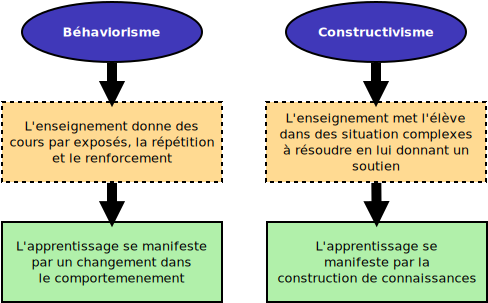
\includegraphics[width=\textwidth]{../resources/illustrations/behaviorisme_constructivisme}
  \caption{Méthode d'apprentissage, béhaviorisme vs. constructivisme}
  \label{fig:behaviorisme_vs_constructivisme_illu}
\end{figure}
\begin{figure}[H]
  \centering
  \includegraphics[width=\textwidth]{../resources/illustrations/behaviorisme_vs_constructivisme}
  \caption{Dessin humoristique, béhaviorisme vs. constructivisme}
  \label{fig:behaviorisme_vs_constructivisme_dessin}
\end{figure}

\subsection{Le constructionnisme}
\begin{minipage}[H]{0.3\linewidth}
  \begin{figure}[H]
  \centering
  \includegraphics[width=0.8\textwidth]{../resources/illustrations/papert}
  \caption{Seymour Papert}
  \end{figure}
\end{minipage}
\begin{minipage}[H]{0.7\linewidth}
Seymour Papert, né en 1928, est informaticien et mathématicien au MIT. Il a créé le groupe de recherche sur l'épistémologie et l'apprentissage au sein du MIT Media Lab, d'où a émergé une théorie de l'apprentissage appelé constructionnisme basée sur la théorie du constructivisme de Piaget\cite{wikipedia_papert}.
\vspace{1cm}
\end{minipage}

Le constructionnisme propose des méthodes favorisant l'apprentissage et la construction de concepts comme proposé dans la théorie de Piaget. Il repose sur quelques notions fondamentales :

\begin{description}
  \item[Le \og Hard Fun \fg{}] : poser des problèmes de manière à ce qu'ils soient perçus comme des Challenges. Il faut confronter les élèves à des problèmes complexes mais réalisables, de manière à ce que leur résolution devienne \og{}fun\fg{}\footnote{\og{}fun\fg{} dans le sens \og{}plaisant\fg{} et non \og drôle \fg{}.} grâce à la difficulté. Cela va créer une forte implication de l'apprenant dans la résolution du problème.
  \item[Interactions] : la notion d'interactions a lieu à deux niveaux. Le premier propose d'effectuer des travaux en groupe, dans le but d'établir des dialogues entre les participants. Le deuxième est l'idée de travailler sur la construction d'une entité réelle, qui peut être observée, commentée et manipulée par autrui.
  \item[Le \og bricolage \fg{}] : introduit par Claude Lévi-Strauss en 1962 dans son livre \emph{La pensée sauvage}, il oppose la science analytique à la science du concret, en dénonçant le fait que la première tend toujours à abstraire les concepts et à instruire une méthode de résolution unique aux élèves. Cette méthode s'oppose au travail dans le concret qui met l'élève face à des difficultés avec peu d'outils. Il devra donc jouer le rôle du \og bricoleur \fg{} en manipulant des objets lui permettant de tendre vers la solution, en \og bricolant \fg{}.
  \item[\og Apprendre à apprendre \fg{} ] : c'est le point résultant des précédents.
\end{description}

\cite{book_seymour_papert}

\begin{coolquote}[Seymour Papert \cite{book_seymour_papert}]
    Le savoir dont les enfants ont le plus besoin est celui qui leur permet d'en acquérir davantage
\end{coolquote}

Seymour Papert voit donc la programmation informatique en groupe comme environnement favorisant les notions énumérées ci-dessus\cite{wikipedia_papert}. En effet de nombreux problèmes peuvent être modélisés et résolus sous cet environnement, le débogage correspondant au \og bricolage \fg{}, et l'entité réelle produite étant le programme créé.

Ainsi, Seymour Papert développa un langage de programmation à but
essentiellement éducatif\footnote{LOGO possède en faite des
  fonctionnalités avancées lui donnant la même puissance qu'un langage
  de programmation \og{}classique\fg{}, mais ses nombreuses primitives
  à visées éducatives et son logo représentant une tortue lui ont valu
  d'être uniquement utilisé à titre éducatif.} : LOGO.

\begin{figure}[H]
  \centering
  \includegraphics[width=.5\textwidth]{../resources/illustrations/logo_logo}
  \caption{Logo de la LOGO Fundation.}
\end{figure}

LOGO à été créé en 1967 puis diffusé largement dans les années 1970. Il est souvent qualifié de \og Lisp sans parenthèses \fg{} et a inspiré de nombreux langages comme NetLogo, SmallTalk, Scratch, etc.

Bien que ses applications éducatives soient variées, trois principales sont énoncées :

\begin{minipage}[H]{0.5\linewidth}
  \begin{description}
    \item[Dessin] : utilisation la plus basique, il est possible de déplacer un curseur afin de tracer des traits à l'écran.
    \item[Turtle] : contrôle de la tortue, qui possède un crayon pour dessiner au sol. L'utilisation est identique à celle du dessin à l'écran.
    \item[Musique] : production musicale, artistique, etc.
  \end{description}
\end{minipage}
\begin{minipage}[H]{0.5\linewidth}
  \begin{figure}[H]
  \flushright
  \includegraphics[width=.9\textwidth]{../resources/illustrations/logo_turtle_1}
  \caption{Seymour Papert et sa Turtle}
  \end{figure}
\end{minipage}

\begin{figure}[H]
  \includegraphics[width=\textwidth]{../resources/illustrations/logo_screen}
  \caption{Déplacements de la tortue possibles.}
\end{figure}

\begin{minipage}[H]{0.5\linewidth}
  \begin{figure}[H]
  \centering
  \includegraphics[width=\textwidth]{../resources/illustrations/logo_turtle_2}
  \caption{Enfants devant la tortue}
  \end{figure}
\end{minipage}
\begin{minipage}[H]{0.5\linewidth}
  \begin{figure}[H]
  \centering
  \includegraphics[width=\textwidth]{../resources/illustrations/logo_turtle_3}
  \caption{Garçon devant la tortue}
  \end{figure}
\end{minipage}

\subsubsection{Versants de l'informatique et de l'éducation}
À l'occasion des 20 ans des conférences EIAH\footnote{Conférences Environnements Informatiques pour l'Apprentissage Humain.}, Seymour Papert, alors conférencier invité, a mis en évidence certains aspects similaires entre informatique et éducation\cite{interview_papert}.

\begin{description}
  \item[L'informatique] a deux fonctions qu'il est nécessaire de distinguer. La première favorise l'accès à l'information via l'utilisation de l'ordinateur et d'internet. Le terme anglais associé est \og Information Technology \fg{}, on peut voir ici l'aspect informationnel de l'informatique. La deuxième est l'utilisation de l'ordinateur dans le but de manipuler des données, par exemple via la programmation informatique. En Anglais \og Computer Science \fg{}, et on parle d'aspect constructionnel de l'informatique.
  \item[L'éducation] propose deux types de contenus différents. Le premier a pour but de délivrer de l'information, comme l'Histoire, la Géographie, le Français, etc. Ces enseignements délivrent des informations qu'il faut savoir. On peut donc parler du côté informationnel de l'éducation. Le deuxième type d'enseignements regroupe tout ce qui gravite autours des Arts, Techniques, Mathématiques, etc. Sont regroupées ici toutes les matières qui travaillent sur la création d'une entité, raisonnement sur des concepts, musique et dessin. On y voit ici l'aspect constructionnel de l'éducation.
\end{description}

Enseigner l'aspect constructionnel énoncé ci-avant requière un environnement complexe à mettre en œuvre. Par exemple, les mathématiques ont permis la construction de pyramides, mais il paraît difficile de permettre aux élèves d’appréhender de nouveaux concepts mathématiques à travers la construction d'une pyramide. Ces enseignements sont donc, pour la plupart, enseignés selon la méthode informationnelle, que l'on peut également nommer méthode analytique (science de l'instruction).

L'informatique et son potentiel à fournir un environnement favorisant la construction d'entités réelles via la programmation et le débogage aurait pu permettre de faciliter le développement de l'aspect constructionnel du système éducatif. Malheureusement les effets furent inverses : l'ordinateur est quasi-exclusivement utilisé dans les écoles et universités comme outil d'aide à la recherche d'informations.

Notons que les applications \og ludiques \fg{} proposées aux élèves ne relèvent pas de l'aspect constructionnel, plaçant l'étudiant dans un rôle d'utilisateur et non de créateur, constructeur et bricoleur.